\section{Test Plan}
In order to test the effectiveness of the filter the mathematical limits, given by the input size and on the coefficient values, had to be tested.
To ease the testing of the filter with different inputs the test-bench inputs and outputs data from/to file.
\subsection{Size limits}
To stress out the size limits computed in section \ref{sec:sizing} the filter was fed with the maximum value in modulus (i.e. $-2^{b-1}= -32768 $) repeated continuously and checked if the output corresponded to the value given by applying in Matlab expression \ref{eq:general} the following graphs are obtained:
\begin{figure}[H]
  \centering
  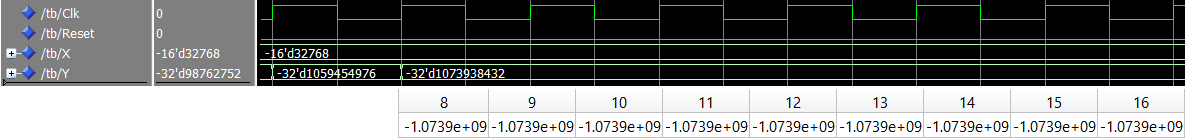
\includegraphics[width=0.9\linewidth]{./images/simul32768.PNG}
  \caption{Test-bench of the filter with -32768 as constant input}
  \label{fig:32768}
\end{figure}
The network at regime settles to -1073938432 that corresponds to the value returned by Matlab.
\subsection{Prove of correctness}
In order to check if the filter performed the convolution expressed in equation \ref{eq:general} a random input was tested and compared against the output of Matlab performing the same operation. The results once the network is at regime are matched by the output produced by Matlab convolution.
\subsection{Filtering}
As input to the network a square wave with a period of 14 samples was given. In Figure \ref{fig:filt} the effect of filtering is highlighted where the first harmonic frequency is kept while other harmonics are cut converging in a sine wave.
\begin{figure}[H]
  \centering
  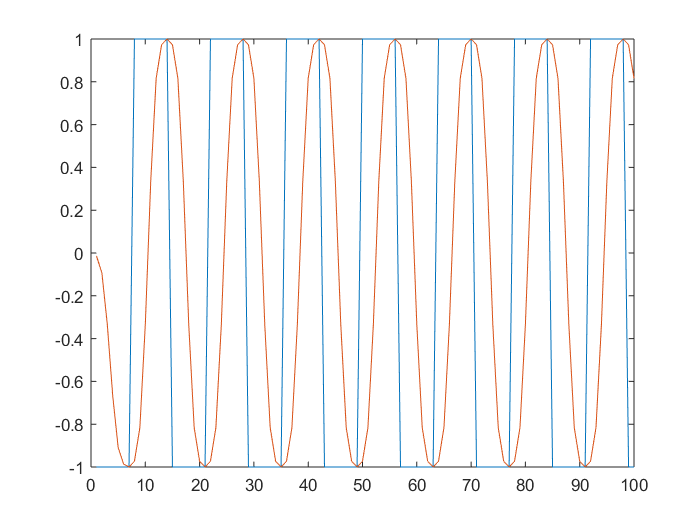
\includegraphics[width=0.9\linewidth]{./images/filtered}
  \caption{Filtered signal in red, input signal in blue}
  \label{fig:filt}
\end{figure}